% Options for packages loaded elsewhere
\PassOptionsToPackage{unicode}{hyperref}
\PassOptionsToPackage{hyphens}{url}
\PassOptionsToPackage{dvipsnames,svgnames,x11names}{xcolor}
%
\documentclass[
  letterpaper,
  DIV=11,
  numbers=noendperiod]{scrartcl}

\usepackage{amsmath,amssymb}
\usepackage{iftex}
\ifPDFTeX
  \usepackage[T1]{fontenc}
  \usepackage[utf8]{inputenc}
  \usepackage{textcomp} % provide euro and other symbols
\else % if luatex or xetex
  \usepackage{unicode-math}
  \defaultfontfeatures{Scale=MatchLowercase}
  \defaultfontfeatures[\rmfamily]{Ligatures=TeX,Scale=1}
\fi
\usepackage{lmodern}
\ifPDFTeX\else  
    % xetex/luatex font selection
\fi
% Use upquote if available, for straight quotes in verbatim environments
\IfFileExists{upquote.sty}{\usepackage{upquote}}{}
\IfFileExists{microtype.sty}{% use microtype if available
  \usepackage[]{microtype}
  \UseMicrotypeSet[protrusion]{basicmath} % disable protrusion for tt fonts
}{}
\makeatletter
\@ifundefined{KOMAClassName}{% if non-KOMA class
  \IfFileExists{parskip.sty}{%
    \usepackage{parskip}
  }{% else
    \setlength{\parindent}{0pt}
    \setlength{\parskip}{6pt plus 2pt minus 1pt}}
}{% if KOMA class
  \KOMAoptions{parskip=half}}
\makeatother
\usepackage{xcolor}
\setlength{\emergencystretch}{3em} % prevent overfull lines
\setcounter{secnumdepth}{-\maxdimen} % remove section numbering
% Make \paragraph and \subparagraph free-standing
\makeatletter
\ifx\paragraph\undefined\else
  \let\oldparagraph\paragraph
  \renewcommand{\paragraph}{
    \@ifstar
      \xxxParagraphStar
      \xxxParagraphNoStar
  }
  \newcommand{\xxxParagraphStar}[1]{\oldparagraph*{#1}\mbox{}}
  \newcommand{\xxxParagraphNoStar}[1]{\oldparagraph{#1}\mbox{}}
\fi
\ifx\subparagraph\undefined\else
  \let\oldsubparagraph\subparagraph
  \renewcommand{\subparagraph}{
    \@ifstar
      \xxxSubParagraphStar
      \xxxSubParagraphNoStar
  }
  \newcommand{\xxxSubParagraphStar}[1]{\oldsubparagraph*{#1}\mbox{}}
  \newcommand{\xxxSubParagraphNoStar}[1]{\oldsubparagraph{#1}\mbox{}}
\fi
\makeatother

\usepackage{color}
\usepackage{fancyvrb}
\newcommand{\VerbBar}{|}
\newcommand{\VERB}{\Verb[commandchars=\\\{\}]}
\DefineVerbatimEnvironment{Highlighting}{Verbatim}{commandchars=\\\{\}}
% Add ',fontsize=\small' for more characters per line
\usepackage{framed}
\definecolor{shadecolor}{RGB}{241,243,245}
\newenvironment{Shaded}{\begin{snugshade}}{\end{snugshade}}
\newcommand{\AlertTok}[1]{\textcolor[rgb]{0.68,0.00,0.00}{#1}}
\newcommand{\AnnotationTok}[1]{\textcolor[rgb]{0.37,0.37,0.37}{#1}}
\newcommand{\AttributeTok}[1]{\textcolor[rgb]{0.40,0.45,0.13}{#1}}
\newcommand{\BaseNTok}[1]{\textcolor[rgb]{0.68,0.00,0.00}{#1}}
\newcommand{\BuiltInTok}[1]{\textcolor[rgb]{0.00,0.23,0.31}{#1}}
\newcommand{\CharTok}[1]{\textcolor[rgb]{0.13,0.47,0.30}{#1}}
\newcommand{\CommentTok}[1]{\textcolor[rgb]{0.37,0.37,0.37}{#1}}
\newcommand{\CommentVarTok}[1]{\textcolor[rgb]{0.37,0.37,0.37}{\textit{#1}}}
\newcommand{\ConstantTok}[1]{\textcolor[rgb]{0.56,0.35,0.01}{#1}}
\newcommand{\ControlFlowTok}[1]{\textcolor[rgb]{0.00,0.23,0.31}{\textbf{#1}}}
\newcommand{\DataTypeTok}[1]{\textcolor[rgb]{0.68,0.00,0.00}{#1}}
\newcommand{\DecValTok}[1]{\textcolor[rgb]{0.68,0.00,0.00}{#1}}
\newcommand{\DocumentationTok}[1]{\textcolor[rgb]{0.37,0.37,0.37}{\textit{#1}}}
\newcommand{\ErrorTok}[1]{\textcolor[rgb]{0.68,0.00,0.00}{#1}}
\newcommand{\ExtensionTok}[1]{\textcolor[rgb]{0.00,0.23,0.31}{#1}}
\newcommand{\FloatTok}[1]{\textcolor[rgb]{0.68,0.00,0.00}{#1}}
\newcommand{\FunctionTok}[1]{\textcolor[rgb]{0.28,0.35,0.67}{#1}}
\newcommand{\ImportTok}[1]{\textcolor[rgb]{0.00,0.46,0.62}{#1}}
\newcommand{\InformationTok}[1]{\textcolor[rgb]{0.37,0.37,0.37}{#1}}
\newcommand{\KeywordTok}[1]{\textcolor[rgb]{0.00,0.23,0.31}{\textbf{#1}}}
\newcommand{\NormalTok}[1]{\textcolor[rgb]{0.00,0.23,0.31}{#1}}
\newcommand{\OperatorTok}[1]{\textcolor[rgb]{0.37,0.37,0.37}{#1}}
\newcommand{\OtherTok}[1]{\textcolor[rgb]{0.00,0.23,0.31}{#1}}
\newcommand{\PreprocessorTok}[1]{\textcolor[rgb]{0.68,0.00,0.00}{#1}}
\newcommand{\RegionMarkerTok}[1]{\textcolor[rgb]{0.00,0.23,0.31}{#1}}
\newcommand{\SpecialCharTok}[1]{\textcolor[rgb]{0.37,0.37,0.37}{#1}}
\newcommand{\SpecialStringTok}[1]{\textcolor[rgb]{0.13,0.47,0.30}{#1}}
\newcommand{\StringTok}[1]{\textcolor[rgb]{0.13,0.47,0.30}{#1}}
\newcommand{\VariableTok}[1]{\textcolor[rgb]{0.07,0.07,0.07}{#1}}
\newcommand{\VerbatimStringTok}[1]{\textcolor[rgb]{0.13,0.47,0.30}{#1}}
\newcommand{\WarningTok}[1]{\textcolor[rgb]{0.37,0.37,0.37}{\textit{#1}}}

\providecommand{\tightlist}{%
  \setlength{\itemsep}{0pt}\setlength{\parskip}{0pt}}\usepackage{longtable,booktabs,array}
\usepackage{calc} % for calculating minipage widths
% Correct order of tables after \paragraph or \subparagraph
\usepackage{etoolbox}
\makeatletter
\patchcmd\longtable{\par}{\if@noskipsec\mbox{}\fi\par}{}{}
\makeatother
% Allow footnotes in longtable head/foot
\IfFileExists{footnotehyper.sty}{\usepackage{footnotehyper}}{\usepackage{footnote}}
\makesavenoteenv{longtable}
\usepackage{graphicx}
\makeatletter
\def\maxwidth{\ifdim\Gin@nat@width>\linewidth\linewidth\else\Gin@nat@width\fi}
\def\maxheight{\ifdim\Gin@nat@height>\textheight\textheight\else\Gin@nat@height\fi}
\makeatother
% Scale images if necessary, so that they will not overflow the page
% margins by default, and it is still possible to overwrite the defaults
% using explicit options in \includegraphics[width, height, ...]{}
\setkeys{Gin}{width=\maxwidth,height=\maxheight,keepaspectratio}
% Set default figure placement to htbp
\makeatletter
\def\fps@figure{htbp}
\makeatother

\KOMAoption{captions}{tableheading}
\makeatletter
\@ifpackageloaded{caption}{}{\usepackage{caption}}
\AtBeginDocument{%
\ifdefined\contentsname
  \renewcommand*\contentsname{Table of contents}
\else
  \newcommand\contentsname{Table of contents}
\fi
\ifdefined\listfigurename
  \renewcommand*\listfigurename{List of Figures}
\else
  \newcommand\listfigurename{List of Figures}
\fi
\ifdefined\listtablename
  \renewcommand*\listtablename{List of Tables}
\else
  \newcommand\listtablename{List of Tables}
\fi
\ifdefined\figurename
  \renewcommand*\figurename{Figure}
\else
  \newcommand\figurename{Figure}
\fi
\ifdefined\tablename
  \renewcommand*\tablename{Table}
\else
  \newcommand\tablename{Table}
\fi
}
\@ifpackageloaded{float}{}{\usepackage{float}}
\floatstyle{ruled}
\@ifundefined{c@chapter}{\newfloat{codelisting}{h}{lop}}{\newfloat{codelisting}{h}{lop}[chapter]}
\floatname{codelisting}{Listing}
\newcommand*\listoflistings{\listof{codelisting}{List of Listings}}
\makeatother
\makeatletter
\makeatother
\makeatletter
\@ifpackageloaded{caption}{}{\usepackage{caption}}
\@ifpackageloaded{subcaption}{}{\usepackage{subcaption}}
\makeatother

\ifLuaTeX
  \usepackage{selnolig}  % disable illegal ligatures
\fi
\usepackage{bookmark}

\IfFileExists{xurl.sty}{\usepackage{xurl}}{} % add URL line breaks if available
\urlstyle{same} % disable monospaced font for URLs
\hypersetup{
  pdftitle={QTM 350 Final},
  pdfauthor={Howie Brown (2585210); Leila Buchan (2550498); Gabe Schwartz (2545628); Tomas Hossain-Aguilar (2582623)},
  colorlinks=true,
  linkcolor={blue},
  filecolor={Maroon},
  citecolor={Blue},
  urlcolor={Blue},
  pdfcreator={LaTeX via pandoc}}


\title{QTM 350 Final}
\author{Howie Brown (2585210) \and Leila Buchan (2550498) \and Gabe
Schwartz (2545628) \and Tomas Hossain-Aguilar (2582623)}
\date{}

\begin{document}
\maketitle


\section{Introduction}\label{introduction}

Gross Domestic Product (GDP) growth serves as a cornerstone of economic
analysis, reflecting the pace at which an economy expands and evolves
over time. A consistently growing GDP is often associated with improved
living standards, increased employment opportunities, and enhanced
government capacity to fund public goods and services. However, the
drivers and correlates of GDP growth are complex and multifaceted, often
intersecting with other critical societal domains such as education.
Education, as a key enabler of human capital development, plays a
pivotal role in sustaining and enhancing economic growth, fostering
innovation, and reducing inequality.

Our project aims to delve into the dynamics of GDP growth by focusing on
the top 20 countries that have exhibited the highest economic growth
rates over the past two decades. By examining this select group, we seek
to uncover patterns and shared characteristics that might illuminate the
factors contributing to their remarkable economic trajectories. Beyond
mere economic performance, our study investigates how these nations have
engaged with education during this period. Specifically, we analyze
their educational engagement, including metrics like school enrollment
rates, literacy levels, and government expenditure on education, to
understand the interplay between economic growth and educational
investment.

To ensure a robust and comprehensive analysis, we utilize data from the
World Bank's World Development Indicators (WDI) database. This extensive
dataset includes over 1,600 indicators spanning 200+ countries from 1960
to 2023, providing a rich foundation for exploring trends in GDP growth
and educational outcomes. By synthesizing these data points, our
research aims to offer nuanced insights into how investments in
education may reinforce or lag behind economic expansion, shedding light
on the long-term sustainability of growth in the world's most rapidly
advancing economies

\section{Data Description}\label{data-description}

The data used in this study is pulled from the World Bank's World
Development Indicators (WDI) database. The dataset contains information
from 200+ countries, with 1,600+ indicators from 1960 to 2023.

Variables used:

\begin{figure}[H]

{\centering \includegraphics{data.png}

}

\caption{Data Selection}

\end{figure}%

\section{Data Analysis}\label{data-analysis}

This shows the line plot of GDP per Capita Growth depending on the year
@gdp-growth-line

\begin{Shaded}
\begin{Highlighting}[]
\ImportTok{import}\NormalTok{ pandas }\ImportTok{as}\NormalTok{ pd}
\ImportTok{import}\NormalTok{ matplotlib.pyplot }\ImportTok{as}\NormalTok{ plt}

\NormalTok{growth\_data }\OperatorTok{=}\NormalTok{ pd.read\_csv(}\StringTok{\textquotesingle{}data/gdp\_growth\_top20.csv\textquotesingle{}}\NormalTok{)}
\NormalTok{growth\_data.drop(columns}\OperatorTok{=}\NormalTok{[}\StringTok{\textquotesingle{}country\_code\textquotesingle{}}\NormalTok{, }\StringTok{\textquotesingle{}avg\_growth\_20yr\textquotesingle{}}\NormalTok{], inplace}\OperatorTok{=}\VariableTok{True}\NormalTok{)}

\CommentTok{\# Melt the DataFrame so that \textquotesingle{}year\textquotesingle{} becomes a variable column and \textquotesingle{}value\textquotesingle{} holds the gdp growth}
\NormalTok{long\_df }\OperatorTok{=}\NormalTok{ growth\_data.melt(id\_vars}\OperatorTok{=}\StringTok{\textquotesingle{}country\textquotesingle{}}\NormalTok{, var\_name}\OperatorTok{=}\StringTok{\textquotesingle{}year\textquotesingle{}}\NormalTok{, value\_name}\OperatorTok{=}\StringTok{\textquotesingle{}gdp\_growth\textquotesingle{}}\NormalTok{)}

\CommentTok{\# Convert \textquotesingle{}year\textquotesingle{} to a numeric type if it\textquotesingle{}s not already}
\NormalTok{long\_df[}\StringTok{\textquotesingle{}year\textquotesingle{}}\NormalTok{] }\OperatorTok{=}\NormalTok{ long\_df[}\StringTok{\textquotesingle{}year\textquotesingle{}}\NormalTok{].astype(}\BuiltInTok{int}\NormalTok{)}

\CommentTok{\# Create the line plot}
\NormalTok{fig, ax }\OperatorTok{=}\NormalTok{ plt.subplots(figsize}\OperatorTok{=}\NormalTok{(}\DecValTok{10}\NormalTok{, }\DecValTok{6}\NormalTok{))}
\NormalTok{ax.tick\_params(axis}\OperatorTok{=}\StringTok{\textquotesingle{}x\textquotesingle{}}\NormalTok{, rotation}\OperatorTok{=}\DecValTok{45}\NormalTok{)}

\CommentTok{\# Group by country and plot each group\textquotesingle{}s data}
\ControlFlowTok{for}\NormalTok{ ctry, grp }\KeywordTok{in}\NormalTok{ long\_df.groupby(}\StringTok{\textquotesingle{}country\textquotesingle{}}\NormalTok{):}
\NormalTok{    color }\OperatorTok{=} \StringTok{\textquotesingle{}black\textquotesingle{}} \ControlFlowTok{if}\NormalTok{ ctry }\OperatorTok{==} \StringTok{\textquotesingle{}World\textquotesingle{}} \ControlFlowTok{else} \VariableTok{None}
\NormalTok{    ax.plot(grp[}\StringTok{\textquotesingle{}year\textquotesingle{}}\NormalTok{], grp[}\StringTok{\textquotesingle{}gdp\_growth\textquotesingle{}}\NormalTok{], label}\OperatorTok{=}\NormalTok{ctry, marker}\OperatorTok{=}\StringTok{\textquotesingle{}o\textquotesingle{}}\NormalTok{, color}\OperatorTok{=}\NormalTok{color)}

\CommentTok{\# Set x{-}axis ticks to integer years}
\NormalTok{years }\OperatorTok{=} \BuiltInTok{sorted}\NormalTok{(long\_df[}\StringTok{\textquotesingle{}year\textquotesingle{}}\NormalTok{].unique())}
\NormalTok{ax.set\_xticks(years)}

\CommentTok{\# Labeling the plot}
\NormalTok{ax.set\_xlabel(}\StringTok{\textquotesingle{}Year\textquotesingle{}}\NormalTok{)}
\NormalTok{ax.set\_ylabel(}\StringTok{\textquotesingle{}GDP per Capita Growth (\%)\textquotesingle{}}\NormalTok{)}
\NormalTok{ax.set\_title(}\StringTok{\textquotesingle{}GDP per Capita Growth Over Time (2003{-}2022)\textquotesingle{}}\NormalTok{)}

\CommentTok{\# Create a legend}
\NormalTok{ax.legend(title}\OperatorTok{=}\StringTok{\textquotesingle{}Country\textquotesingle{}}\NormalTok{, bbox\_to\_anchor}\OperatorTok{=}\NormalTok{(}\FloatTok{1.05}\NormalTok{, }\DecValTok{1}\NormalTok{), loc}\OperatorTok{=}\StringTok{\textquotesingle{}upper left\textquotesingle{}}\NormalTok{)}

\NormalTok{plt.tight\_layout()}
\NormalTok{plt.show()}
\end{Highlighting}
\end{Shaded}

\begin{figure}[H]

{\centering 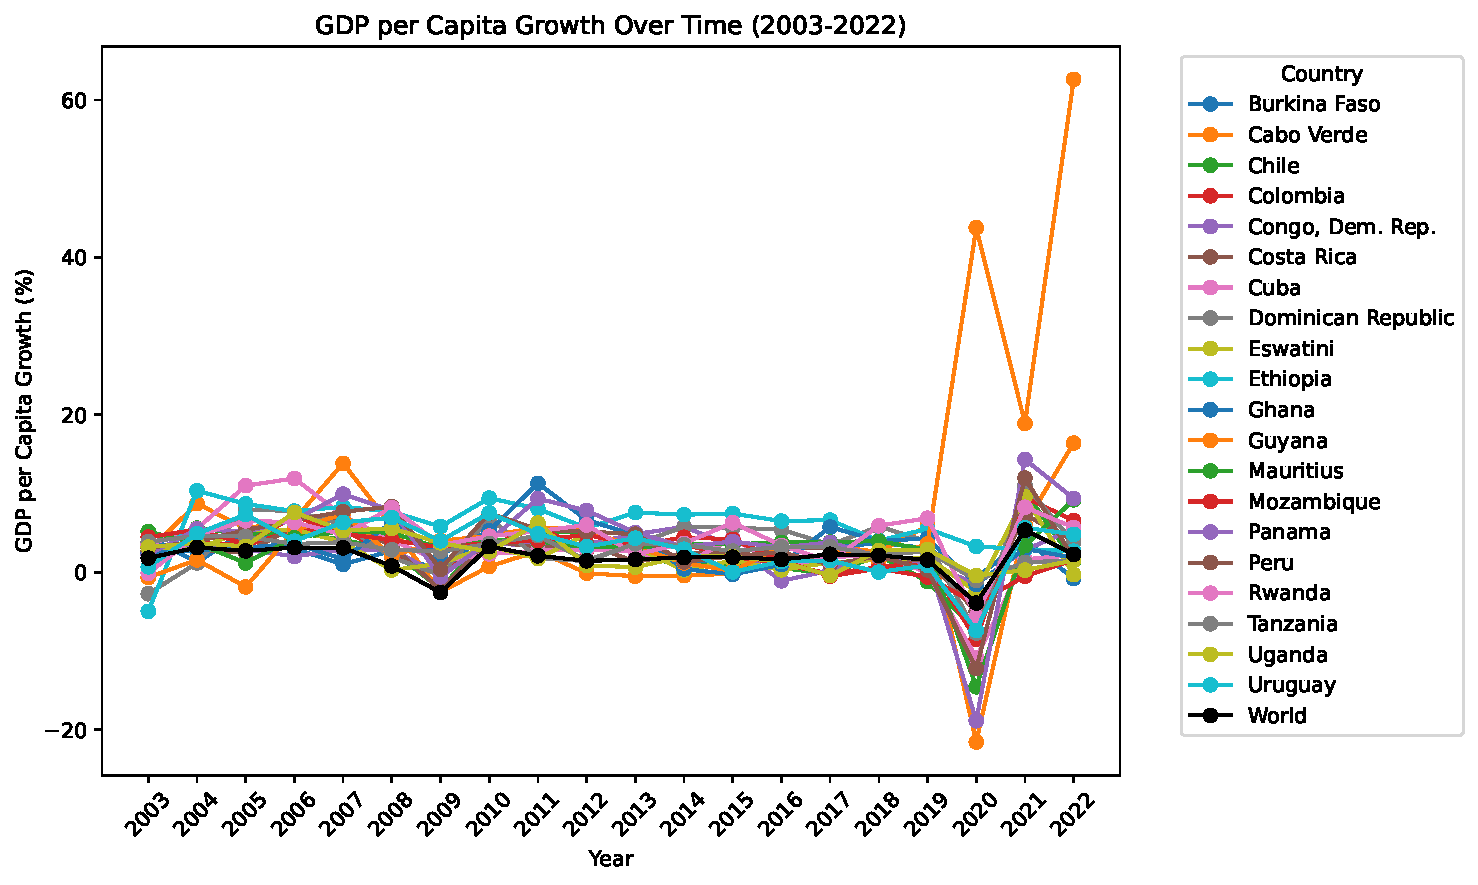
\includegraphics{report_files/figure-pdf/gdp-growth-line-output-1.pdf}

}

\caption{GDP per Capita Growth Line Plot}

\end{figure}%

This shows the bar graph of GDP per Capita Growth depending on the
countries @gdp-growth-hist

\begin{Shaded}
\begin{Highlighting}[]
\ImportTok{import}\NormalTok{ pandas }\ImportTok{as}\NormalTok{ pd}
\ImportTok{import}\NormalTok{ matplotlib.pyplot }\ImportTok{as}\NormalTok{ plt}

\CommentTok{\# Read the data}
\NormalTok{data }\OperatorTok{=}\NormalTok{ pd.read\_csv(}\StringTok{\textquotesingle{}data/gdp\_growth\_top20.csv\textquotesingle{}}\NormalTok{)}

\CommentTok{\# Extract the global average (World)}
\NormalTok{world\_avg }\OperatorTok{=}\NormalTok{ data.loc[data[}\StringTok{\textquotesingle{}country\textquotesingle{}}\NormalTok{] }\OperatorTok{==} \StringTok{\textquotesingle{}World\textquotesingle{}}\NormalTok{, }\StringTok{\textquotesingle{}avg\_growth\_20yr\textquotesingle{}}\NormalTok{].values[}\DecValTok{0}\NormalTok{]}

\CommentTok{\# Filter out the \textquotesingle{}World\textquotesingle{} row from the DataFrame so we only have the top 20 countries}
\NormalTok{data\_countries }\OperatorTok{=}\NormalTok{ data[data[}\StringTok{\textquotesingle{}country\textquotesingle{}}\NormalTok{] }\OperatorTok{!=} \StringTok{\textquotesingle{}World\textquotesingle{}}\NormalTok{]}

\NormalTok{fig, ax }\OperatorTok{=}\NormalTok{ plt.subplots(figsize}\OperatorTok{=}\NormalTok{(}\DecValTok{12}\NormalTok{, }\DecValTok{6}\NormalTok{))}

\CommentTok{\# Create a bar plot with countries on the x{-}axis and avg\_growth\_20yr on the y{-}axis}
\NormalTok{ax.bar(data\_countries[}\StringTok{\textquotesingle{}country\textquotesingle{}}\NormalTok{], data\_countries[}\StringTok{\textquotesingle{}avg\_growth\_20yr\textquotesingle{}}\NormalTok{], color}\OperatorTok{=}\StringTok{\textquotesingle{}skyblue\textquotesingle{}}\NormalTok{)}

\CommentTok{\# Add a horizontal line at the global average}
\NormalTok{ax.axhline(y}\OperatorTok{=}\NormalTok{world\_avg, color}\OperatorTok{=}\StringTok{\textquotesingle{}red\textquotesingle{}}\NormalTok{, linestyle}\OperatorTok{=}\StringTok{\textquotesingle{}{-}{-}\textquotesingle{}}\NormalTok{, label}\OperatorTok{=}\SpecialStringTok{f\textquotesingle{}World Avg: }\SpecialCharTok{\{}\NormalTok{world\_avg}\SpecialCharTok{:.2f\}}\SpecialStringTok{\%\textquotesingle{}}\NormalTok{)}

\CommentTok{\# Rotate x{-}axis labels for better readability}
\NormalTok{plt.xticks(rotation}\OperatorTok{=}\DecValTok{45}\NormalTok{, ha}\OperatorTok{=}\StringTok{\textquotesingle{}right\textquotesingle{}}\NormalTok{)}

\CommentTok{\# Add labels and title}
\NormalTok{plt.xlabel(}\StringTok{\textquotesingle{}Country\textquotesingle{}}\NormalTok{)}
\NormalTok{plt.ylabel(}\StringTok{\textquotesingle{}Average GDP Growth (20{-}year)\textquotesingle{}}\NormalTok{)}
\NormalTok{plt.title(}\StringTok{\textquotesingle{}Top 20 Countries by Average GDP Per Capita Growth vs. Global Average\textquotesingle{}}\NormalTok{)}

\CommentTok{\# Add legend}
\NormalTok{ax.legend()}
\NormalTok{plt.tight\_layout()}
\NormalTok{plt.show()}
\end{Highlighting}
\end{Shaded}

\begin{figure}[H]

{\centering 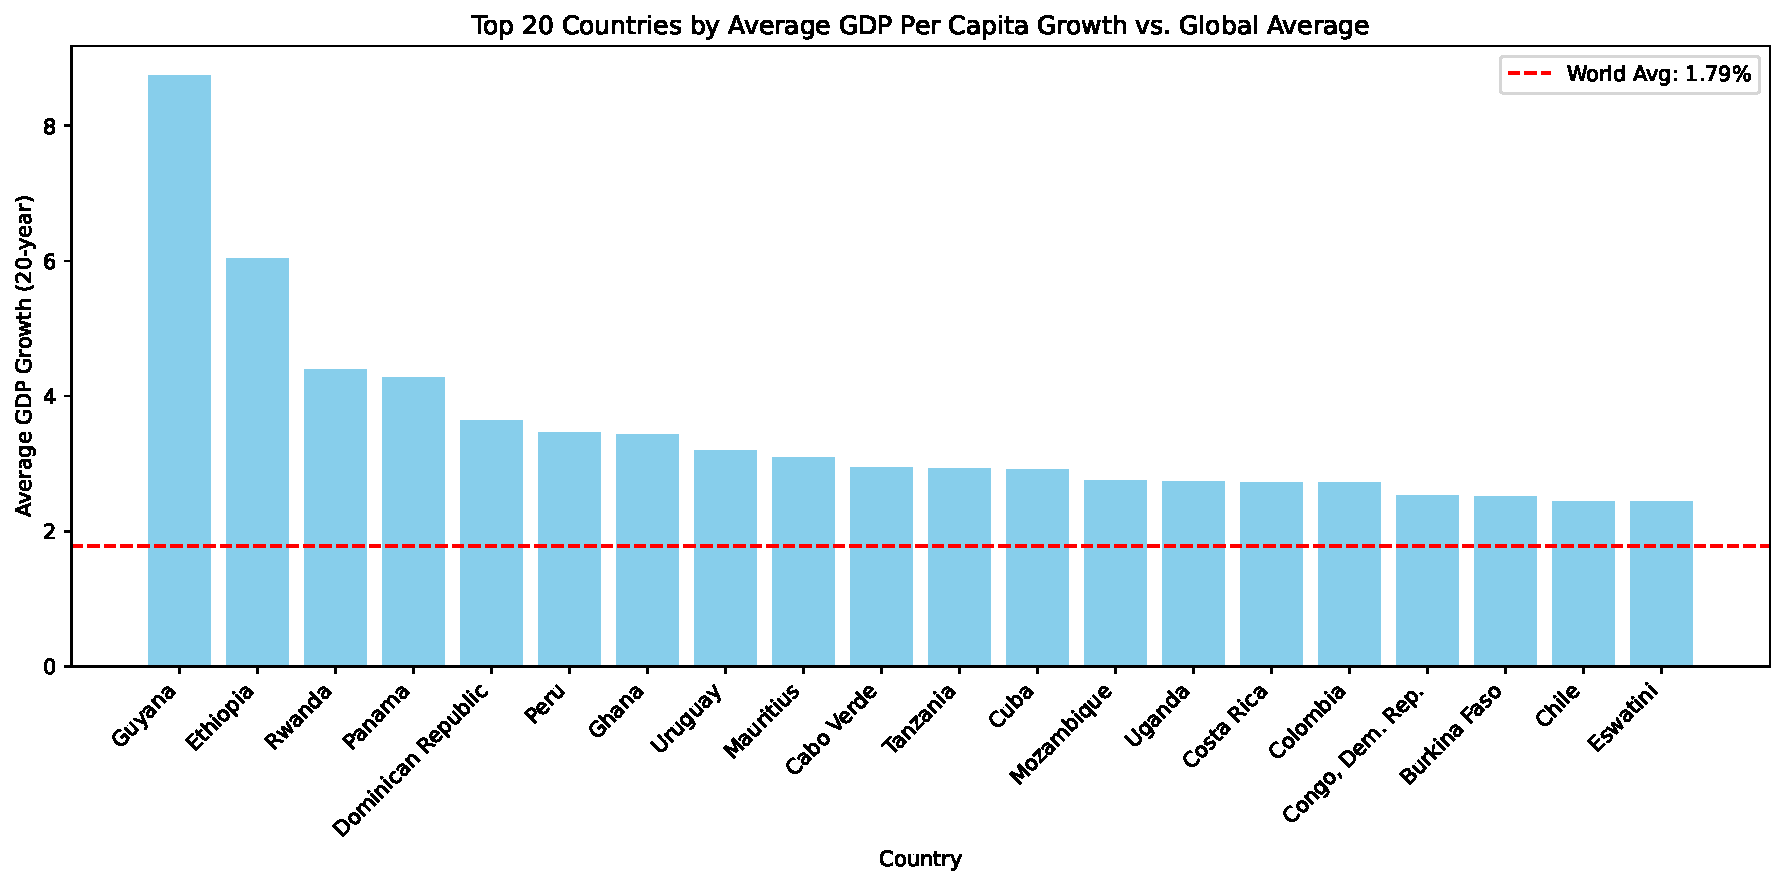
\includegraphics{report_files/figure-pdf/gdp-growth-hist-output-1.pdf}

}

\caption{GDP per Capita Growth Bar Chart}

\end{figure}%

The correlation heatmap showing the complex relationship between average
GDP growth, enrollment growth at primary/secondary and tertiary levels,
and educational expenditure growth @correlation

\begin{Shaded}
\begin{Highlighting}[]
\ImportTok{import}\NormalTok{ pandas }\ImportTok{as}\NormalTok{ pd}
\ImportTok{import}\NormalTok{ matplotlib.pyplot }\ImportTok{as}\NormalTok{ plt}
\ImportTok{import}\NormalTok{ seaborn }\ImportTok{as}\NormalTok{ sns}

\NormalTok{df }\OperatorTok{=}\NormalTok{ pd.read\_csv(}\StringTok{"data/averaged\_full.csv"}\NormalTok{)}

\NormalTok{corr\_matrix }\OperatorTok{=}\NormalTok{ df.drop(columns}\OperatorTok{=}\NormalTok{[}\StringTok{\textquotesingle{}year\textquotesingle{}}\NormalTok{]).corr()}

\BuiltInTok{print}\NormalTok{(corr\_matrix)}

\NormalTok{plt.figure(figsize}\OperatorTok{=}\NormalTok{(}\DecValTok{16}\NormalTok{, }\DecValTok{12}\NormalTok{))}
\NormalTok{sns.heatmap(corr\_matrix, annot}\OperatorTok{=}\VariableTok{True}\NormalTok{, cmap}\OperatorTok{=}\StringTok{\textquotesingle{}coolwarm\textquotesingle{}}\NormalTok{)}
\NormalTok{plt.title(}\StringTok{\textquotesingle{}Correlation Between Growth in GDP per Capita vs. Primary and Secondary Schooling}\CharTok{\textbackslash{}n}\StringTok{Enrollment Rates on Average\textquotesingle{}}\NormalTok{)}
\NormalTok{plt.show()}
\end{Highlighting}
\end{Shaded}

\begin{verbatim}
                                avg_gdp_growth  avg_enrollment_growth  \
avg_gdp_growth                        1.000000               0.190227   
avg_enrollment_growth                 0.190227               1.000000   
avg_tertiary_enrollment_growth        0.302815               0.494932   
avg_expenditure_on_edu_growth        -0.109279              -0.064807   

                                avg_tertiary_enrollment_growth  \
avg_gdp_growth                                        0.302815   
avg_enrollment_growth                                 0.494932   
avg_tertiary_enrollment_growth                        1.000000   
avg_expenditure_on_edu_growth                         0.053655   

                                avg_expenditure_on_edu_growth  
avg_gdp_growth                                      -0.109279  
avg_enrollment_growth                               -0.064807  
avg_tertiary_enrollment_growth                       0.053655  
avg_expenditure_on_edu_growth                        1.000000  
\end{verbatim}

\begin{figure}[H]

{\centering 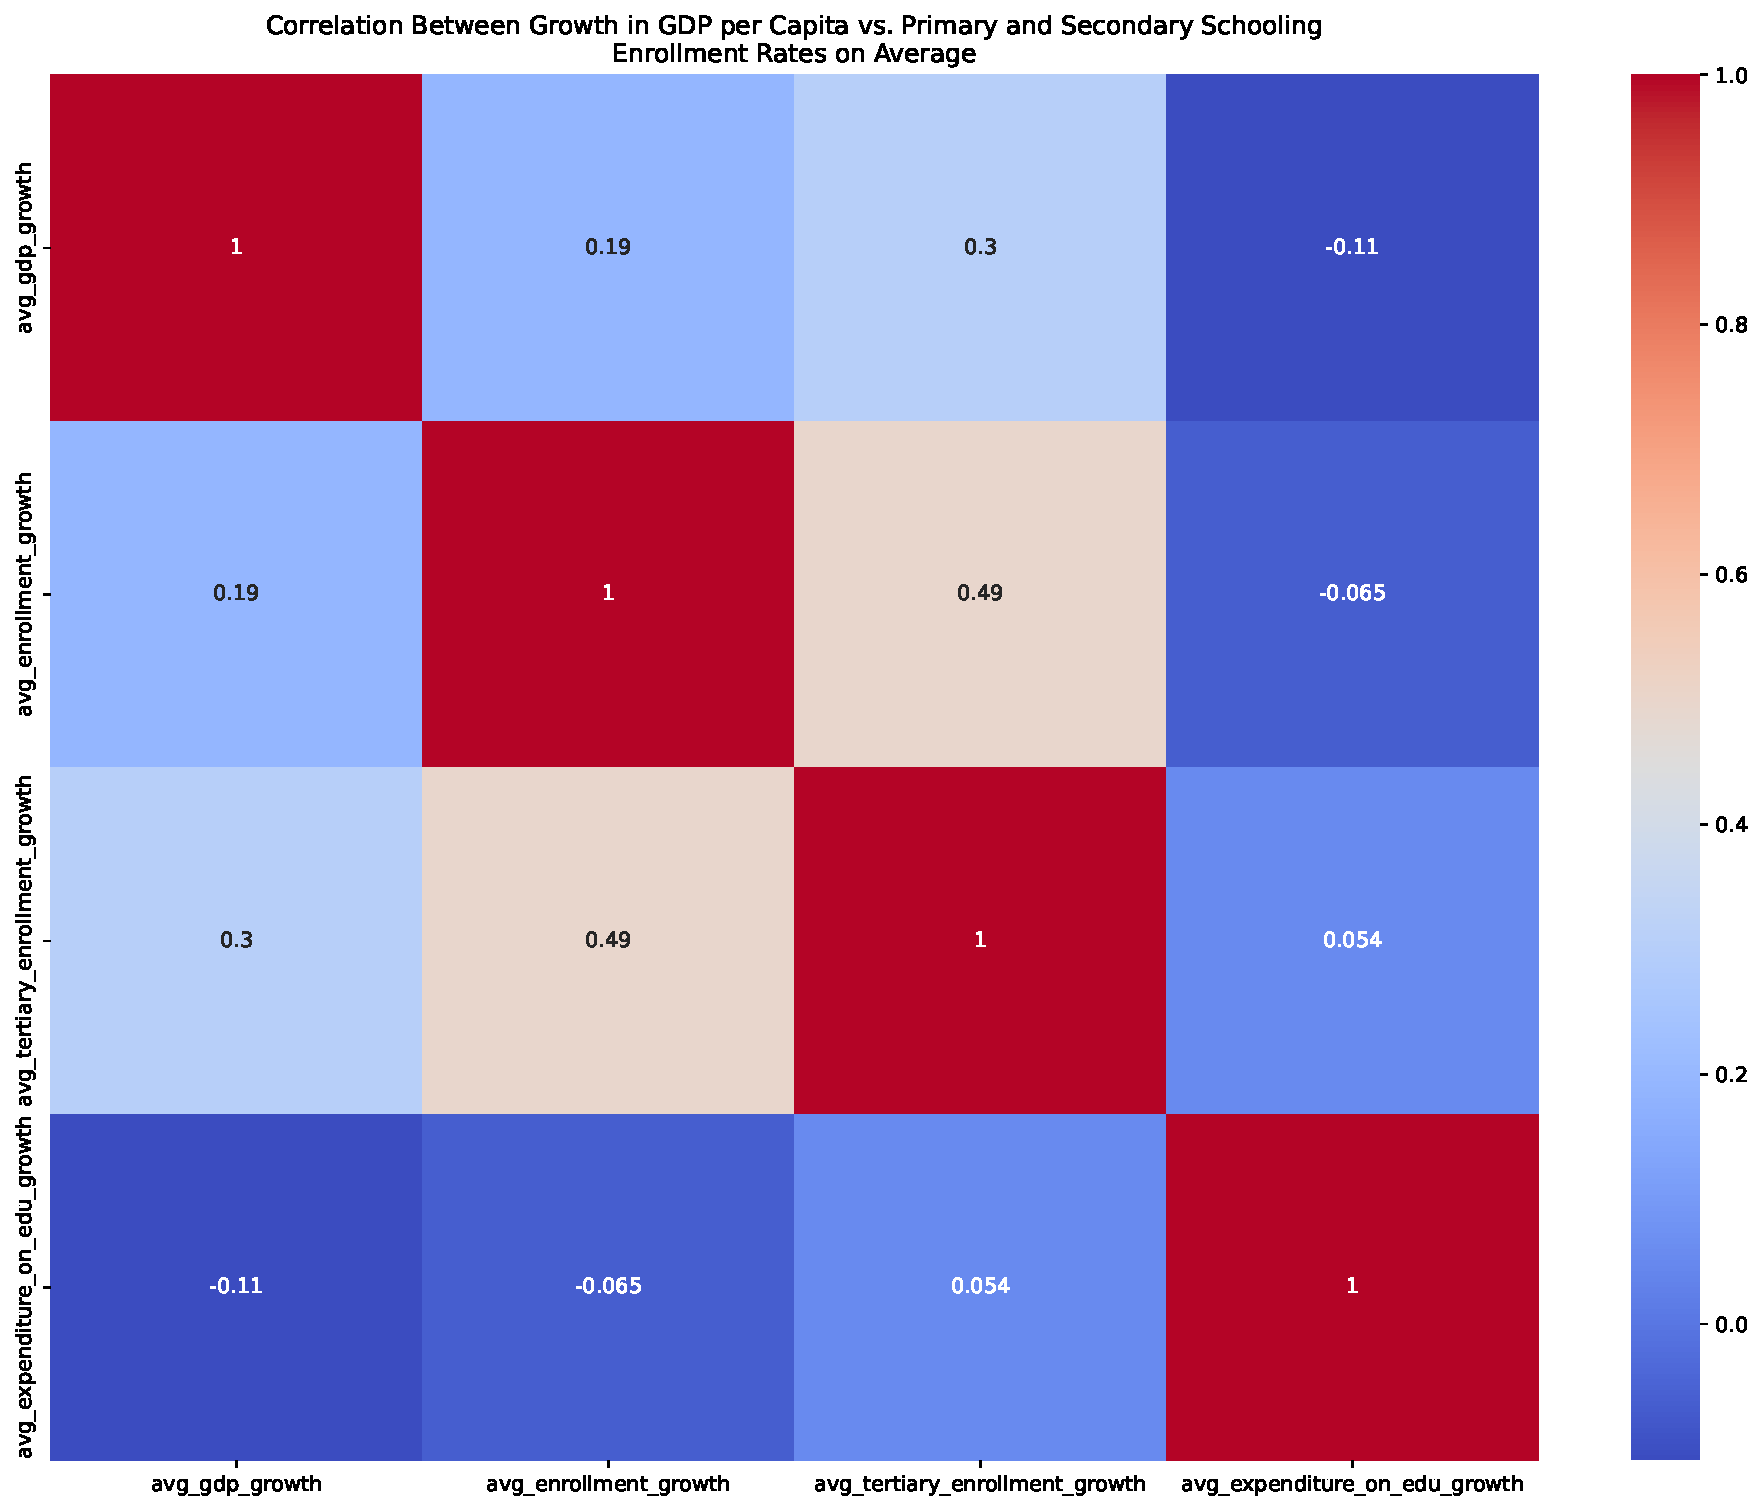
\includegraphics{report_files/figure-pdf/correlation-output-2.pdf}

}

\caption{GDP per Capita Growth vs Education Enrollment Matrix}

\end{figure}%

\section{Results and Discussions}\label{results-and-discussions}

For figure 1, most countries closely tracked the global (World) trend in
GDP per capita growth from 2003 to 2022, showing steady moderate
increases until a steep drop around 2020, coinciding with the onset of
the COVID-19 pandemic. This dip is evident across nearly all lines,
reflecting the worldwide economic disruption. While most countries
rebounded similarly to the global average, one or two outliers diverged
significantly, showing sharp spikes in subsequent years. Overall, about
18 of the 20 countries followed patterns largely consistent with the
global trend, with COVID-19 causing a clear, temporary plunge in growth
rates. Except for Guyana which experienced a large GDP increase during
this pandemic due to oil offshoring (World Bank).

For figure 2, the bar chart shows the top 20 countries by their average
20-year GDP per capita growth rates, compared against the global average
of 1.79\%. The same pattern is seen here where Guyana leads by a wide
margin, followed by Ethiopia and Rwanda, all substantially outperforming
the global benchmark. The rest of the top 20 countries also have
consistently higher growth rates than the world average, reflecting how
strong the growth in these countries has been. This visualization makes
it easier to see which country is which and which has more growth than
others, however it is impossible to see the year by year trend for each
country.

Lastly for figure 3, while GDP growth shows modest positive correlations
with enrollment growth (0.19) and tertiary enrollment growth (0.3),
while these links are relatively weak, it does suggest that there is
some effect of increase in higher education on growth in GDP . In fact,
the correlation between GDP growth and education expenditure growth is
slightly negative (-0.16), implying that increased education spending
does not immediately translate into economic gains. Within the education
indicators themselves, a moderate correlation (0.47) between enrollment
growth and tertiary enrollment growth indicates some alignment, but the
generally low correlations between expenditure and other educational
metrics indicate that funding alone does not guarantee improved
outcomes. Overall, these findings underscore the complexity of
translating educational inputs into broader economic benefits and
suggest that policymakers need holistic strategies that target
efficiency, alignment of resources, and long-term development goals.

\section{Conclusions}\label{conclusions}

In this study, we set out to explore the relationship between economic
growth and educational engagement by focusing on the top 20 countries
with the highest GDP growth rates over the past two decades. The WDI
required meticulous data cleaning to ensure accuracy and relevance,
including handling missing values, standardizing metrics, and isolating
the variables most pertinent to our research. To facilitate our analysis
and present the results, we employed multiple visualization strategies
to display the findings from the data. We used a line plot to show the
difference between GDP per capita growth in the 20 selected countries
over the past 20 years, compared to the world average GDP per capita
growth. Second, a bar chart compares the same metric but as an average
over the course of the two decades. Finally, a correlation matrix
offered an in-depth view of the relationships between economic and
educational variables, such as GDP growth, school enrollment rates, and
educational expenditure. This matrix allowed us to identify significant
positive or negative correlations and assess the strength of these
relationships.

We utilized Python and PostgreSQL to fetch country-level primary and
secondary school enrollment data for the years 2002--2022, averaged
missing values using forward and backward filling, filtered countries
with at least 15 years of data, and then computed and exported both the
average enrollments and their year-over-year growth rates to CSV files.
We applied a similar strategy to calculate the tertiary enrollment rate
in these countries. To calculate expenditures, we created code that
retrieved education expenditure as a percentage of GDP from a PostgreSQL
database, stored the raw data to a CSV file, filtered countries that had
at least 15 years of data, used forward filling to handle missing
values, then calculated the year-over-year percentage growth in
expenditure for each country and saved the final results to another CSV
file. To access the GDP data, we first filtered countries to those with
limited missing data, imputed missing values using their row-averages,
calculated each country's average 20-year growth, and selected the top
20 performing countries along with the ``World'' data for context. After
retrieving and attaching country codes, we saved the resulting table to
CSV files and also inserted it into a PostgreSQL database, creating the
necessary table if it did not exist.

Finally we took these four datasets (GDP growth, enrollment growth,
tertiary enrollment growth, and educational expenditure growth), removed
all unwanted columns, and then averaged each metric across all remaining
countries by year. After aligning column names, these yearly averages
are combined side-by-side into a single DataFrame, resulting in a tidy
table that shows the average growth values for all metrics by year.

Overall, our analysis shows that while most countries broadly mirrored
the world's pattern of moderate GDP growth followed by a
pandemic-induced downturn, a few outliers like Guyana diverged
dramatically due to unique economic factors. Educational variables, such
as enrollment rates and expenditure, demonstrated only weak correlations
with GDP growth, indicating that these factors alone may not drive
economic performance. Ultimately, these findings highlight the
multifaceted nature of economic development and the need for
comprehensive strategies that go beyond simply increasing educational
inputs to achieve sustainable growth.




\end{document}
